\chapter{Módulo de contabilidad}
\label{ref:capituloV}\section{El libro mayor}
\section{El libro diario}
\subsubsection{Asignando apuntes a partidas}
\label{ref:asignarapuntepartida}La asignación de apuntes a partidas
permite generar de forma automática la plantilla de justificación
de gastos e ingresos que vuestra financiadora suele exigir a la
finalización del mismo. Esta plantilla se ha definido dentro del
proyecto como has visto en el apartado  del capítulo .



\begin{center}
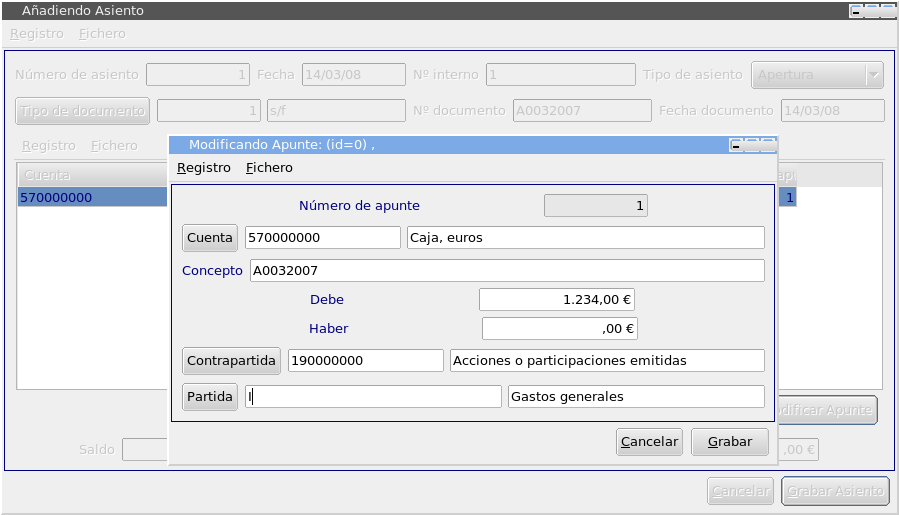
\includegraphics[width=11.299cm,height=6.606cm]{manual-img23.png}
\end{center}

\bigskip


\bigskip


\bigskip


\bigskip


\bigskip


\bigskip


\bigskip


\bigskip


\bigskip


\bigskip


\bigskip

